\section{Framework}
\subsection{Introduction}


\subsection{Supply-chain Levels for Software Artifacts}
\acrlong{slsa}\footnote{Available at: https://slsa.dev/} is a framework for securing the software supply chain created by Google in collaboration with OpenSSF\footnote{Available at: https://openssf.org/}. The framework is made into a common vocabulary checklist for developers to evaluate the security of the software they are creating. \acrshort{slsa} is organized into tracks and levels. The levels refer to the increasing security guarantee of the supply chain, the highest level being level 3. The levels are split further into tracks. Tracks are certain aspects of the supply chain, for example, the Build track, which currently is \acrshort{slsa}s only track. \cite{SLSAgeneral}

\vspace{2mm}
\begin{figure}[H]
    \centering
    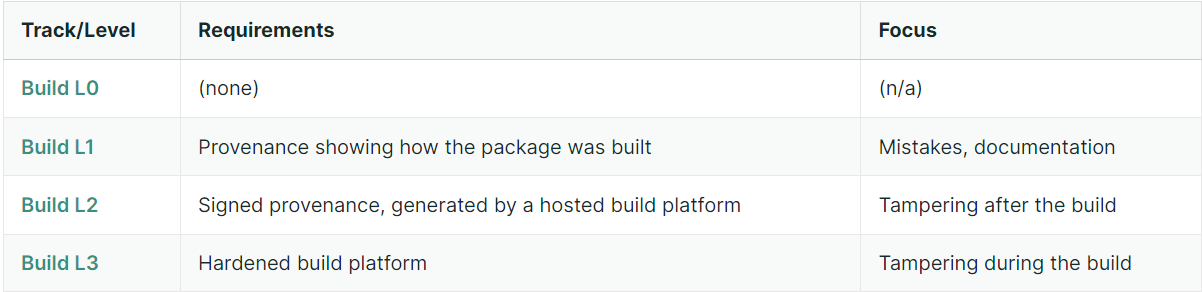
\includegraphics[width=0.8\columnwidth]{Images/slsalevels.png}
    \caption{SLSA levels for the Build track} Adapted from: \cite{SLSAlevels}
    \label{fig: SLSA levels for the Build track}
\end{figure}

Currently, there are three levels split into one track. To achieve the different build levels, the developers have to do the following:
\\~\\
To achieve \acrshort{slsa} Build Level 1, the developers are required to use a consistent build process, which can easily be adopted. Additionally, the build platform has to generate \gls{provenance} automatically, which describes how the artifact was built. This includes information on the entity responsible for building the package, the specific build process used, and the top-level inputs utilized during the build process.
\\~\\
To achieve \acrshort{slsa} Level 2, all Level 1 requirements must be in place. Further, the build has to be run on a platform that generates signs the \gls{provenance}. This \gls{provenance}'s authenticity also has to be verified.
\\~\\
Similarly to Level 2, all previous level requirements have to be achieved to get to \acrshort{slsa} Level 3. In addition, the build platform has to have controls to secure the secrets used for signing \gls{provenance}and prevent runs from the same project impact each other. 


\subsection{Secure Software Development Framework}
\acrlong{ssdf}\footnote{Latest version: https://nvlpubs.nist.gov/nistpubs/SpecialPublications/NIST.SP.800-218.pdf} is a framework consisting of practices for a secure software development, created by \acrlong{nist}. The company should integrate the \acrshort{ssdf} into their already existing software development practices. SSDF does not specify how each practice should be implemented. It emphasizes the outcome of the practices rather than how to perform them. Organizations in any sector or community can use the SSDF, regardless of their size or level of cybersecurity competence. This framework is intended to be user-friendly and adaptable, making it appropriate for a wide range of businesses with varied levels of cybersecurity knowledge. Organizations can use the SSDF to adopt secure software development practices and reduce the risk of potential security vulnerabilities. The framework does not introduce new practices or define new terminology, but it rather presents a set of high-level practices that are based on known standards, guidelines, and documents relevant to secure software development practices. 

The benefits of describing the practices at a high level include that they can be used by organizations in every industry and community, despite their size or level of cybersecurity knowledge. It can also help companies that buy and use software to understand the secure software development methods used by the suppliers they work with. 

The practices are separated into four groups:
\begin{itemize}
  \item \textbf{Prepare the Organization (PO)}: \say{Organizations should ensure that their people, processes, and technology are prepared to perform secure software development at the organization level. Many organizations will find some PO practices to also be applicable to subsets of their software development, like individual development groups or projects.}  
  
  \item Protect the Software (PS)
  \item Produce Well-Secured Software (PW)
  \item Respond to Vulnerabilities (RV)
\end{itemize}

Each practice definition has the following components:
\begin{itemize}
  \item \textbf{Practice}: name of the practice with a unique identifier, with a description of the practice 
  \item \textbf{Task}: One or more steps that may be required to carry out a procedure
  \item \textbf{Notional Implementation Examples}: Examples of tools, procedures, or approaches that can help in task implementation are offered, although they are not complete nor required. Some examples may not be relevant to specific companies or circumstances.
  \item \textbf{References}: References towards established secure development practice documentation and their mappings to specific tasks. Not all references will be relevant in all cases of software development. \cite{ssdf}
\end{itemize}




